% !TeX TS-program = pdflatex
% !BIB TS-program = biber
\documentclass[aspectratio=169]{beamer}
\documentclass[border=1pt]{standalone}
% packages
\usepackage{tikz}
\usepackage{tikz-qtree}
\usetikzlibrary{positioning,quotes,calc,arrows.meta,shapes}
% tikz setup
\tikzset{%
  arrow/.style = {
    ->,
    > = latex,
    very thick,
    rounded corners,
    fill = #1,
    draw = #1,
  },
  wide/.style = {
    line width = #1,
  },
  tbox/.style = {
    thick,
    rounded corners,
    fill = #1!20!white,
    draw = #1!80!white,
    align = center,
    minimum width = 0.8cm,
    minimum height = 0.6cm,
    node distance = 1.5cm,
  },
  branch/.style = {
    grow = down,
    thick,
    rounded corners = 0.1cm,
    fill = #1!20!white,
    draw = #1!80!white,
    align = center,
    minimum width = 3cm,
    minimum height = 1cm,
    node distance = 1cm,
  },
  branch/.default = {gray},
  leaf/.style = {
    grow = down,
    thick,
    rounded corners = 0.35cm,
    fill = #1!20!white,
    draw = #1!80!white,
    align = center,
    minimum width = 0.7cm,
    minimum height = 0.7cm,
    font = \normalfont,
  },
  leaf/.default = {blue},
}
% selectors
\definecolor{all}     {RGB}{  0,  0,  0}
\definecolor{S}       {RGB}{  0,153,255}
\definecolor{I}       {RGB}{204, 51,  0}
\definecolor{T}       {RGB}{204, 51,153}
\definecolor{infected}{RGB}{204,  0, 51}
\definecolor{High}    {RGB}{ 34, 34, 34}
\definecolor{Med}     {RGB}{ 85, 85, 85}
\definecolor{Low}     {RGB}{187,187,187}
% from beamer
\definecolor{C1}{HTML}{224466}
\definecolor{C2}{HTML}{CC3300}
\definecolor{C3}{HTML}{666666}

\documentclass[border=1pt]{standalone}
% packages
\usepackage{tikz}
\usepackage{tikz-qtree}
\usetikzlibrary{positioning,quotes,calc,arrows.meta,shapes}
% tikz setup
\tikzset{%
  arrow/.style = {
    ->,
    > = latex,
    very thick,
    rounded corners,
    fill = #1,
    draw = #1,
  },
  wide/.style = {
    line width = #1,
  },
  tbox/.style = {
    thick,
    rounded corners,
    fill = #1!20!white,
    draw = #1!80!white,
    align = center,
    minimum width = 0.8cm,
    minimum height = 0.6cm,
    node distance = 1.5cm,
  },
  branch/.style = {
    grow = down,
    thick,
    rounded corners = 0.1cm,
    fill = #1!20!white,
    draw = #1!80!white,
    align = center,
    minimum width = 3cm,
    minimum height = 1cm,
    node distance = 1cm,
  },
  branch/.default = {gray},
  leaf/.style = {
    grow = down,
    thick,
    rounded corners = 0.35cm,
    fill = #1!20!white,
    draw = #1!80!white,
    align = center,
    minimum width = 0.7cm,
    minimum height = 0.7cm,
    font = \normalfont,
  },
  leaf/.default = {blue},
}
% selectors
\definecolor{all}     {RGB}{  0,  0,  0}
\definecolor{S}       {RGB}{  0,153,255}
\definecolor{I}       {RGB}{204, 51,  0}
\definecolor{T}       {RGB}{204, 51,153}
\definecolor{infected}{RGB}{204,  0, 51}
\definecolor{High}    {RGB}{ 34, 34, 34}
\definecolor{Med}     {RGB}{ 85, 85, 85}
\definecolor{Low}     {RGB}{187,187,187}
% from beamer
\definecolor{C1}{HTML}{224466}
\definecolor{C2}{HTML}{CC3300}
\definecolor{C3}{HTML}{666666}

\title[Influence of risk group turnover under assortative mixing]
      {Influence of simulated risk group turnover\\
       in STI epidemics with assortative mixing}
\author{Jesse Knight, Sharmistha Mishra}
\github{github.com/mishra-lab/turnover}
\institute{Institute of Medical Science\\University of Toronto}
\date{\textbf{Canadian Student Health Research Forum}\\[0.5em]\scriptsize
  2020 August 25}
\titlegraphic{\flushright\vspace{-0.7\textheight}\documentclass{article}
\usepackage{underscore,relsize,bm,mathtools,amssymb}
\usepackage[margin=2cm]{geometry}
\usepackage{tikz}
\usepackage[colorlinks,linkcolor=blue]{hyperref}

\setlength{\parindent}{0pt}
\setlength{\parskip}{6pt}
\setlength{\skip\footins}{1cm}
\newcommand{\N}{\textsc{n}}
\newcommand{\hreftt}[1]{\href{#1}{\texttt{#1}}}
\usepackage{listings}
\lstset{language=Python}
\lstdefinestyle{Python}{
    language        = Python,
    basicstyle      = \ttfamily\footnotesize,
    keywordstyle    = [1]\color[rgb]{0.0,0.4,0.8},
    keywordstyle    = [2]\color[rgb]{0.9,0.6,0.3},
    stringstyle     = \color[rgb]{0.7,0.2,0.6},
    commentstyle    = \color[rgb]{0.2,0.8,0.5}
}
\lstset{
  columns          = full,
  frame            = single,
  rulecolor        = \color{gray},
  numbers          = left,
  numberstyle      = \ttfamily\color[rgb]{0.8,0.8,0.8},
  showstringspaces = false,
}


\title{\vspace{-1.2cm}Automatically Computing Turnover\\for Steady-State Population Distributions}
\author{Jesse Knight}
\date{July 16, 2018\\\footnotesize{Revision 1: October 9, 2018\\[-1em]}}
%%%%%%%%%%%%%%%%%%%%%%%%%%%%%%%%%%%%%%%%%%%%%%%%%%%%%%%%%%%%%%%%%%%%%%%%%%%%%%%%%%%%%%%%%%%%%%%%%%%%
\begin{document}
%%%%%%%%%%%%%%%%%%%%%%%%%%%%%%%%%%%%%%%%%%%%%%%%%%%%%%%%%%%%%%%%%%%%%%%%%%%%%%%%%%%%%%%%%%%%%%%%%%%%
\maketitle
%%%%%%%%%%%%%%%%%%%%%%%%%%%%%%%%%%%%%%%%%%%%%%%%%%%%%%%%%%%%%%%%%%%%%%%%%%%%%%%%%%%%%%%%%%%%%%%%%%%%
\section{Background}
When modelling sexually transmitted diseases, 
it is important to consider heterogeneity in levels of sexual activity among the population,
as transmission dynamics are profoundly impacted by these characteristics.
Moreover, it is rarely sufficient to model static groups,
since people's sexual behaviour typically changes over time.
Therefore, transfer of individuals between activity groups should be included in the model,
which we call ``turnover''.
\par
The most important implications of this feature are the transfer of
\textit{infected} and \textit{susceptible} individuals
from one activity group to another,
which provides another mode of transmission besides
direct sexual contact between the activity groups.%
\footnote{An interesting parallel can be found with the modes of heat transfer:
  conduction -- direct transfer of heat by particles in contact
  (contact within an activity group),
  versus 
  convection -- movement of hot particles from one area to another
  (turnover).}
For example, in a perfectly assortative population,
activity level turnover is the only way transmission can occur \textit{between} activity groups.
\par
From the modelling perspective,
it is possible to consider turnover from any group to any other group.
However, the definition of turnover rates among each of the groups
will impact the steady-state population distribution.
So too will the rates of births and deaths,
and the distribution of new individuals. Our problem, then, is as follows:
\par
\textbf{Problem:} How do we choose turnover rates,
in conjunction with rates of birth and death, and the distribution of entering individuals,
in order to yield a specific steady-state distribution of activity levels in the population?
\par
\textbf{Hypothesis:} There exists a closed-form equation relating these rates and distributions.
\par
\textbf{Application:} This equation can be used to define
the appropriate rates of population turnover,
in order to match the other observed parameters.
%%%%%%%%%%%%%%%%%%%%%%%%%%%%%%%%%%%%%%%%%%%%%%%%%%%%%%%%%%%%%%%%%%%%%%%%%%%%%%%%%%%%%%%%%%%%%%%%%%%%
\section{Maths}
We denote the state variable representing
the proportion of the population in activity group $i \in [1 \dots \N]$ as $x_i$
and the vector of all $x_i$ as $\bm{x}$.
Since turnover transitions can occur between any two groups, in either direction,
we denote the turnover rates as an $\N \times \N$ matrix $\zeta$,
where $\zeta_{ij}$ corresponds to the transition $x_i \rightarrow x_j$.
A verbose definition is given in Eq.~(\ref{eq:zeta}),
where the diagonal elements are denoted $*$ since they are not useful.
\begin{equation}\label{eq:zeta}
\zeta = \left[\begin{array}{cccc}
	         *           & x_1  \rightarrow x_2 & \cdots & x_1 \rightarrow x_\N \\[0.5em]
	x_2  \rightarrow x_1 &          *           & \cdots & x_2 \rightarrow x_\N \\[0.5em]
	      \vdots         &       \vdots         & \ddots &       \vdots         \\[0.5em]
	x_\N \rightarrow x_1 & x_\N \rightarrow x_2 & \cdots &          *
\end{array}\right]
\end{equation}
The rate of population entry is denoted $\nu$, and exit as $\mu$.
The proportion of the entering population who are activity level $i$ is denoted $p_i$,
while the distribution of exiting population is simply $x_i$.
\par
These transitions and related rates are summarized for $\N = 3$ in Figure \ref{fig:turnover}.
\par
Our aim now is to relate these quantities to
a target steady-state distribution for the vector $\bm{x}$.
\begin{figure}
  \centering
  \usetikzlibrary{positioning,arrows.meta,quotes,calc}
\tikzset{%
  arrow/.style    = { ->, >=Latex,  line width = 0.4mm, rounded corners, draw = black, every edge/.style={arrow} },
  arrow/.style    = { ->, >=Latex,  very thick, rounded corners, draw = black,
    fill = #1, draw = #1, font = \footnotesize },
  tbox/.style     = { fill = #1!20!white, draw = #1!80!white, thick, align = center,
    minimum width = 1cm, node distance = 1.5cm }
}
\newcommand{\connectall}[2]{
  \foreach \s in {#1} {
    \foreach \t in {#2} {
      \draw[arrow,<->] (\s) -- (\t);
    }
  }
}

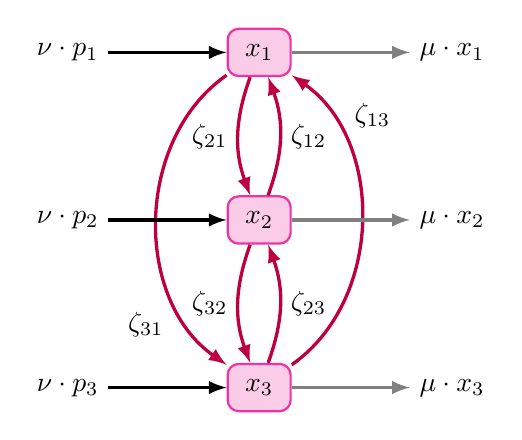
\begin{tikzpicture}
\node(i1) [tbox=magenta] at (0.0,0.0)    {$x_1$};
\node(i2) [tbox=magenta, below = of i1]  {$x_2$};
\node(i3) [tbox=magenta, below = of i2]  {$x_3$};
\node(b1) [left  = 1.5cm of i1] {$\nu \cdot p_1$};
\node(b2) [left  = 1.5cm of i2] {$\nu \cdot p_2$};
\node(b3) [left  = 1.5cm of i3] {$\nu \cdot p_3$};
\node(d1) [right = 1.5cm of i1] {$\mu \cdot x_1$};
\node(d2) [right = 1.5cm of i2] {$\mu \cdot x_2$};
\node(d3) [right = 1.5cm of i3] {$\mu \cdot x_3$};

\draw[arrow=purple] (i1) edge["$\zeta_{21}$", swap, bend right=20] (i2); 
\draw[arrow=purple] (i2) edge["$\zeta_{12}$", swap, bend right=20] (i1);
\draw[arrow=purple] (i3) edge["$\zeta_{23}$", swap, bend right=20] (i2); 
\draw[arrow=purple] (i2) edge["$\zeta_{32}$", swap, bend right=20] (i3);
\draw[arrow=purple] (i1) edge["$\zeta_{31}$", swap, bend right=55, near end] (i3); 
\draw[arrow=purple] (i3) edge["$\zeta_{13}$", swap, bend right=55, near end] (i1);
\draw[arrow=black]  (b1) -- (i1);
\draw[arrow=black]  (b2) -- (i2);
\draw[arrow=black]  (b3) -- (i3);
\draw[arrow=gray]   (i1) -- (d1);
\draw[arrow=gray]   (i2) -- (d2);
\draw[arrow=gray]   (i3) -- (d3);
\end{tikzpicture}
  \caption{Schematic of demographic transitions among 3 activity groups:
    high $x_1$, medium $x_2$, low $x_3$;
    entry is shown in black,
    exit is shown in grey,
    turnover is shown in purple.}%
  \label{fig:turnover}
\end{figure}
% ==================================================================================================
\subsection{System Equations}
For a given activity level, the rate of change of the group is defined by the net flows, as in:
\begin{equation}
  \frac{d}{dt}x_i
= \nu \thinspace p_i + \sum_{j}{\zeta_{ji} \thinspace x_j}
%- \mu \thinspace x_i - \sum_{j}{\zeta_{ij} \thinspace x_i} % confusing...
- x_i \left( \mu + \sum_{j}{\zeta_{ij}} \right) % ugly
\end{equation}
In matrix form, we can write the entire system as:
\begin{equation}\label{eq:sys-dxdt}
  \frac{d}{dt}\bm{x}
= \nu \thinspace \bm{p} + \left(\bm{x}^{\mathsf{T}} \zeta\right)
- \bm{x} \left( \mu + \sum_{j}{\zeta_{ij}} \right)
\end{equation}
Let's assume that $\nu$, $\mu$, and $\bm{p}$ are known,
and that we aim to find $\zeta$ which yields
the observed distribution of activity levels $\bm{x}$ at equilibrium.
At equilibrium, the derivative may not actually be zero, however,
since populations typically grow over time at a rate $g = \nu - \mu$.
The desired equilibrium rate of change is therefore given by
$\nu\thinspace\bm{x} - \mu\thinspace\bm{x}$,
which we can substitute for the left hand side of Eq.~(\ref{eq:sys-dxdt})
and rearrange to give:%
\footnote{Note that this system does not depend on $\mu$.}
\begin{equation}
\nu (\bm{x} - \bm{p}) =
\left(\bm{x}^{\mathsf{T}} \zeta\right) - \bm{x} \sum_{j}{\zeta_{ij}}
\end{equation}
The right hand side can then be factored to give
a linear system of $\bm{z} = \mathrm{vec}(\zeta)$, parametrized by $\bm{x}$:
\begin{equation}\label{eq:y=Az}
\nu (\bm{x} - \bm{p}) =
A \thinspace \bm{z}, \qquad
A \in \mathbb{R}^{\N \times \N^2}, \enspace A_{ij} = f(x,i,j)
\end{equation}
Some example systems showing the linear factorization $A$ and $\bm{z}$
are given in \nameref{ap:eg-sys},
while \nameref{ap:code} gives an algorithm for defining $A$ for any $\N$.
% ==================================================================================================
\subsection{Solving the System}
While it is possible to solve Eq.~(\ref{eq:y=Az}), a number of problems emerge.
\begin{enumerate}
  \item \textbf{Diagonal elements}\label{prob:diag} --
  The diagonal elements of $\zeta$ have no impact on the system.
  Therefore in any solution, they will be undefined.
  \item \textbf{Underdetermined system}\label{prob:rank} --
  For $\N > 2$, the system is underdetermined,
  since $\mathrm{Rank}(A) = \N \le (\N\times\N - \N)$.
  This means that A is not invertible and
  there are many possible solutions to $\bm{b} = A\bm{z}$.
  \item \textbf{Bounding $\bm{\zeta}$}\label{prob:bounds} --
  Exact solution methods to this problem do not permit consideration of nonlinear constraints.
  Importantly, this includes bounds on the values of $\zeta$,
  which must not be negative or excessively large.
\end{enumerate}
Problem \ref{prob:diag} is actually trivial,
as the diagonal values of $\zeta$ can simply be
removed from the system before solving, then set to zero post-hoc,
as in \nameref{ap:code}.
\par
Problem \ref{prob:rank} can also be solved easily using $\bm{z} = A^{+}\bm{b}$,
where $A^{+}$ denotes the pseudo-inverse of $A$:
\begin{equation}
A^{+} = A^{\mathsf{T}}{\left(A \thinspace A^{\mathsf{T}}\right)}^{-1}
\end{equation}
This approach additionally minimizes the L2-norm of $\bm{z}$,
which provides the necessary constraints to find a unique solution directly.
In this case, smaller values of $\zeta$ are also desirable,
since high levels of turnover are not expected,
and smaller values afford stability to the model.
\par
Problem \ref{prob:bounds}, however, unfortunately precludes the use of
direct solution methods like $\bm{z} = A^{+}\bm{b}$,
since bounds on $x_i$ are not enforceable in these approaches.
Still, many other (iterative) techniques for solving the system exist.
In \nameref{ap:code}, the Limited-memory BFGS algorithm for bounded problems%
\footnote{Courtesy of the
  \href{https://docs.scipy.org/doc/scipy-1.0.0/reference/generated/scipy.optimize.minimize.html}%
       {\texttt{optimize.minimize}}
  function from SciPy.}
is used to minimize $\mathcal{J}(\bm{z}) = {\left|\left| A\bm{z} - \bm{b} \right|\right|}_2$,
subject to bounds $l \le z_i \le u, \enspace\forall i$,
providing a solution $\bm{z}$, which is reshaped to give $\zeta$.
\par
It should be noted that such optimizations should converge to zero, not just a small number,
since the system is still underdetermined.
Any other final values of $\mathcal{J}$ likely indicate convergence problems,
and may result in model instability due to unbalanced transitions.
% ==================================================================================================
\subsection{Additional Constraints}
One advantage of the proposed framework is that
it is simple to add additional constraints on $\zeta$
of the form $\bm{b}' = A' \thinspace \bm{z}$;
these constraints can simply be appended to $\bm{b}$ and the rows of $A$ as in:
\begin{equation}
\left[\begin{array}{c} \bm{b}\\\bm{b}' \end{array}\right]
=
\left[\begin{array}{c}     A \\    A ' \end{array}\right]
\end{equation}
Using the notation $n_{ij}$ to represent the vectorized index $ij$ so that
$z_{n_{ij}} = \zeta_{ij}$,
here are some examples:
\begin{itemize}
  \item If one specific transition rate $\zeta_{ij} = r$ is known, append:
  \begin{gather}
    \left[\begin{array}{c} r \end{array}\right] =
    \left[\begin{array}{ccc} e_{1} & \cdots & e_{\N^2} \end{array}\right]
    \shortintertext{where}
    e_{n} = \begin{cases}
    1 & n = n_{ij}\\
    0 & \mathrm{else}
    \end{cases}
  \end{gather}
  \item If the average duration in a given activity class $d_{i}$ is known, append:
  \begin{gather}
    \left[\begin{array}{c} {d_{i}}^{-1} - \mu \end{array}\right] =
    \left[\begin{array}{ccc} e_{1} & \cdots & e_{\N^2} \end{array}\right]
    \shortintertext{where}
    e_{n} = \begin{cases}
    1 & n = n_{ij},\enspace j\in [1,\dots,\N] \\
    0 & \mathrm{else}
    \end{cases}\nonumber
    \shortintertext{since}
    d_k = {\left( \mu + \sum_{j}{\zeta_{kj}} \right)}^{-1}
  \end{gather}
  \item If a crude control over the overall magnitude of turnover is desired
  (L1-norm of $\zeta$ = $Z$), append:
  \begin{equation}
    \left[\begin{array}{c} Z \end{array}\right] =
    \left[\begin{array}{ccc} 1 & \cdots & 1 \end{array}\right]
  \end{equation}
\end{itemize}
The necessary number of additional constraints to yield
a fully determined system is $\N\times\N - 2\thinspace\N$.
While it is possible to construct such a system for a given $\N$,
most sets of constraints won't easily fill this gap for any $\N$.
For example, specifying the durations for all activity levels $\bm{d}$
yields $\N$ additional constraints.
For $\N = 3$, this happily yields a unique solution,
but for $\N = 4$, we will still have $(\N\times\N - 2\thinspace\N) - \N = 4$ degrees of freedom,
and so on.
Still, this flexibility can certainly be useful to better match any available data.
%%%%%%%%%%%%%%%%%%%%%%%%%%%%%%%%%%%%%%%%%%%%%%%%%%%%%%%%%%%%%%%%%%%%%%%%%%%%%%%%%%%%%%%%%%%%%%%%%%%%
\section{Conclusion}
We have resolved a relationship between some typically available demographic parameters
and rates of group turnover $\zeta$ which yield a particular steady-state distribution.
This allows us to compute $\zeta$ on the fly,
as shown in the \texttt{zetafun} function in \nameref{ap:code}.
Additional linear constraints can be considered when solving for $\zeta$,
represented by the optional arguments \texttt{bprime} and \texttt{Aprime} to \texttt{zetafun}.
Bounds on $\zeta$ can also be considered (e.g.\ \texttt{bounds}),
depending on the method used to solve the system.
\par
Finally, it should be noted that the analysis here has not considered
disease-attributable death,
a potentially serious limitation.
Methods to ensure demographic stability in the face of significant disease-attributable death,
or even if it is suitable to do so,
should be the subject of future work.
%%%%%%%%%%%%%%%%%%%%%%%%%%%%%%%%%%%%%%%%%%%%%%%%%%%%%%%%%%%%%%%%%%%%%%%%%%%%%%%%%%%%%%%%%%%%%%%%%%%%
\clearpage\section*{Appendix A: Example Systems}\label{ap:eg-sys}
Here we show examples of the system:
\begin{equation}
\nu (\bm{x} - \bm{p}) = A \thinspace \bm{z}
\end{equation}
for $\N = 2$ and $\N = 3$.
% ==================================================================================================
\subsection*{$\bm{\mathrm{N}}$ = 2}
\begin{equation}
\left[\begin{array}{c}
\nu (x_1 - p_1) \\
\nu (x_2 - p_2) 
\end{array}\right]
= 
\left[\begin{array}{cccc}
\cdot & -x_1  &  x_2  & \cdot \\
\cdot &  x_1  & -x_2  & \cdot
\end{array}\right]
\left[\begin{array}{c}
\zeta_{11} \\ \zeta_{12} \\ \zeta_{21} \\ \zeta_{22}
\end{array}\right]
\end{equation}
% ==================================================================================================
\subsection*{$\bm{\mathrm{N}}$ = 3}
\begin{equation}
\left[\begin{array}{c}
\nu (x_1 - p_1) \\
\nu (x_2 - p_2) \\
\nu (x_3 - p_3) 
\end{array}\right]
= 
\left[\begin{array}{ccccccccc}
\cdot & -x_1  & -x_1  &  x_2  & \cdot & \cdot &  x_3  & \cdot & \cdot \\
\cdot &  x_1  & \cdot & -x_2  & \cdot & -x_2  & \cdot &  x_3  & \cdot \\
\cdot & \cdot &  x_1  & \cdot & \cdot &  x_2  & -x_3  & -x_3  & \cdot 
\end{array}\right]
\left[\begin{array}{c}
\zeta_{11} \\ \zeta_{12} \\ \zeta_{13} \\ \zeta_{21} \\ \zeta_{22} \\ \zeta_{23} \\ \zeta_{31} \\ \zeta_{32} \\ \zeta_{33}
\end{array}\right]
\end{equation}
%%%%%%%%%%%%%%%%%%%%%%%%%%%%%%%%%%%%%%%%%%%%%%%%%%%%%%%%%%%%%%%%%%%%%%%%%%%%%%%%%%%%%%%%%%%%%%%%%%%%
\clearpage\section*{Appendix B: Python Code}\label{ap:code}
\lstinputlisting[style=Python]{py/turnover.py}
\textbf{Result}:
\lstinputlisting[style=Python]{py/result.txt}
%%%%%%%%%%%%%%%%%%%%%%%%%%%%%%%%%%%%%%%%%%%%%%%%%%%%%%%%%%%%%%%%%%%%%%%%%%%%%%%%%%%%%%%%%%%%%%%%%%%%
\end{document}}
\begin{document}
% ------------------------------------------------------------------------------
\begin{frame}
  \maketitle
\end{frame}
\begin{frame}
  \paragraph{Disclosures}
  \xpar
  None
  \vfill
  \paragraph{Acknowledgements}
  \xpar
  \newcommand{\xlogo}[2]{\raisebox{-0.5\height}{~\includegraphics[height=#1em]{#2}}~}
\begin{equation*}
\begin{array}{ccccccc}
  \xlogo{2.4}{cihr}  &
  \xlogo{2.4}{nserc} &
  \xlogo{1.7}{map}   &
  \xlogo{2.2}{smh}   &
  \xlogo{2.4}{uoft}
\end{array}
\end{equation*}
\end{frame}
% ==============================================================================
\section{Introduction}
% ------------------------------------------------------------------------------
\begin{frame}{Background}
  \pause
  \visible<+->{
  \textbc{STI} ---
  \textit{Sexually Transmitted Infections}
  \begin{itemize}
    \item 1+ million new STI infections per day\footcite{Rowley2019}
    \item 1.7 million new HIV infections per year\footcite{AIDSinfo}
  \end{itemize}}
  \xpar
  \visible<+->{
  \textbc{tPAF} ---
  \textit{Transmission Population Attributable Fraction}\footcite{Mishra2014}
  \begin{itemize}
    \item based on epidemic simulation models
    \item \% onward infections from unmet needs of risk group $\rightarrow$ inform interventions
  \end{itemize}}
\end{frame}
% ------------------------------------------------------------------------------
\begin{frame}{Key Modelling Concepts}
  \tikzpausetrue\vspace{-1em}
  \begin{columns}[t]
    \begin{column}<+->{0.5\linewidth}
      \visible<+->{\paragraph{Turnover:} movement between risk groups}
      \visible<+->{\xpar\centering\documentclass{article}
\usepackage{underscore,relsize,bm,mathtools,amssymb}
\usepackage[margin=2cm]{geometry}
\usepackage{tikz}
\usepackage[colorlinks,linkcolor=blue]{hyperref}

\setlength{\parindent}{0pt}
\setlength{\parskip}{6pt}
\setlength{\skip\footins}{1cm}
\newcommand{\N}{\textsc{n}}
\newcommand{\hreftt}[1]{\href{#1}{\texttt{#1}}}
\usepackage{listings}
\lstset{language=Python}
\lstdefinestyle{Python}{
    language        = Python,
    basicstyle      = \ttfamily\footnotesize,
    keywordstyle    = [1]\color[rgb]{0.0,0.4,0.8},
    keywordstyle    = [2]\color[rgb]{0.9,0.6,0.3},
    stringstyle     = \color[rgb]{0.7,0.2,0.6},
    commentstyle    = \color[rgb]{0.2,0.8,0.5}
}
\lstset{
  columns          = full,
  frame            = single,
  rulecolor        = \color{gray},
  numbers          = left,
  numberstyle      = \ttfamily\color[rgb]{0.8,0.8,0.8},
  showstringspaces = false,
}


\title{\vspace{-1.2cm}Automatically Computing Turnover\\for Steady-State Population Distributions}
\author{Jesse Knight}
\date{July 16, 2018\\\footnotesize{Revision 1: October 9, 2018\\[-1em]}}
%%%%%%%%%%%%%%%%%%%%%%%%%%%%%%%%%%%%%%%%%%%%%%%%%%%%%%%%%%%%%%%%%%%%%%%%%%%%%%%%%%%%%%%%%%%%%%%%%%%%
\begin{document}
%%%%%%%%%%%%%%%%%%%%%%%%%%%%%%%%%%%%%%%%%%%%%%%%%%%%%%%%%%%%%%%%%%%%%%%%%%%%%%%%%%%%%%%%%%%%%%%%%%%%
\maketitle
%%%%%%%%%%%%%%%%%%%%%%%%%%%%%%%%%%%%%%%%%%%%%%%%%%%%%%%%%%%%%%%%%%%%%%%%%%%%%%%%%%%%%%%%%%%%%%%%%%%%
\section{Background}
When modelling sexually transmitted diseases, 
it is important to consider heterogeneity in levels of sexual activity among the population,
as transmission dynamics are profoundly impacted by these characteristics.
Moreover, it is rarely sufficient to model static groups,
since people's sexual behaviour typically changes over time.
Therefore, transfer of individuals between activity groups should be included in the model,
which we call ``turnover''.
\par
The most important implications of this feature are the transfer of
\textit{infected} and \textit{susceptible} individuals
from one activity group to another,
which provides another mode of transmission besides
direct sexual contact between the activity groups.%
\footnote{An interesting parallel can be found with the modes of heat transfer:
  conduction -- direct transfer of heat by particles in contact
  (contact within an activity group),
  versus 
  convection -- movement of hot particles from one area to another
  (turnover).}
For example, in a perfectly assortative population,
activity level turnover is the only way transmission can occur \textit{between} activity groups.
\par
From the modelling perspective,
it is possible to consider turnover from any group to any other group.
However, the definition of turnover rates among each of the groups
will impact the steady-state population distribution.
So too will the rates of births and deaths,
and the distribution of new individuals. Our problem, then, is as follows:
\par
\textbf{Problem:} How do we choose turnover rates,
in conjunction with rates of birth and death, and the distribution of entering individuals,
in order to yield a specific steady-state distribution of activity levels in the population?
\par
\textbf{Hypothesis:} There exists a closed-form equation relating these rates and distributions.
\par
\textbf{Application:} This equation can be used to define
the appropriate rates of population turnover,
in order to match the other observed parameters.
%%%%%%%%%%%%%%%%%%%%%%%%%%%%%%%%%%%%%%%%%%%%%%%%%%%%%%%%%%%%%%%%%%%%%%%%%%%%%%%%%%%%%%%%%%%%%%%%%%%%
\section{Maths}
We denote the state variable representing
the proportion of the population in activity group $i \in [1 \dots \N]$ as $x_i$
and the vector of all $x_i$ as $\bm{x}$.
Since turnover transitions can occur between any two groups, in either direction,
we denote the turnover rates as an $\N \times \N$ matrix $\zeta$,
where $\zeta_{ij}$ corresponds to the transition $x_i \rightarrow x_j$.
A verbose definition is given in Eq.~(\ref{eq:zeta}),
where the diagonal elements are denoted $*$ since they are not useful.
\begin{equation}\label{eq:zeta}
\zeta = \left[\begin{array}{cccc}
	         *           & x_1  \rightarrow x_2 & \cdots & x_1 \rightarrow x_\N \\[0.5em]
	x_2  \rightarrow x_1 &          *           & \cdots & x_2 \rightarrow x_\N \\[0.5em]
	      \vdots         &       \vdots         & \ddots &       \vdots         \\[0.5em]
	x_\N \rightarrow x_1 & x_\N \rightarrow x_2 & \cdots &          *
\end{array}\right]
\end{equation}
The rate of population entry is denoted $\nu$, and exit as $\mu$.
The proportion of the entering population who are activity level $i$ is denoted $p_i$,
while the distribution of exiting population is simply $x_i$.
\par
These transitions and related rates are summarized for $\N = 3$ in Figure \ref{fig:turnover}.
\par
Our aim now is to relate these quantities to
a target steady-state distribution for the vector $\bm{x}$.
\begin{figure}
  \centering
  \usetikzlibrary{positioning,arrows.meta,quotes,calc}
\tikzset{%
  arrow/.style    = { ->, >=Latex,  line width = 0.4mm, rounded corners, draw = black, every edge/.style={arrow} },
  arrow/.style    = { ->, >=Latex,  very thick, rounded corners, draw = black,
    fill = #1, draw = #1, font = \footnotesize },
  tbox/.style     = { fill = #1!20!white, draw = #1!80!white, thick, align = center,
    minimum width = 1cm, node distance = 1.5cm }
}
\newcommand{\connectall}[2]{
  \foreach \s in {#1} {
    \foreach \t in {#2} {
      \draw[arrow,<->] (\s) -- (\t);
    }
  }
}

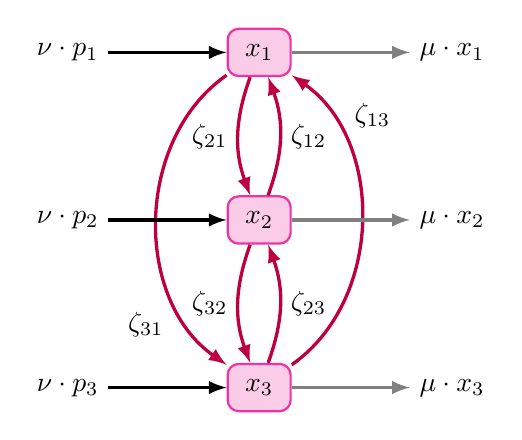
\begin{tikzpicture}
\node(i1) [tbox=magenta] at (0.0,0.0)    {$x_1$};
\node(i2) [tbox=magenta, below = of i1]  {$x_2$};
\node(i3) [tbox=magenta, below = of i2]  {$x_3$};
\node(b1) [left  = 1.5cm of i1] {$\nu \cdot p_1$};
\node(b2) [left  = 1.5cm of i2] {$\nu \cdot p_2$};
\node(b3) [left  = 1.5cm of i3] {$\nu \cdot p_3$};
\node(d1) [right = 1.5cm of i1] {$\mu \cdot x_1$};
\node(d2) [right = 1.5cm of i2] {$\mu \cdot x_2$};
\node(d3) [right = 1.5cm of i3] {$\mu \cdot x_3$};

\draw[arrow=purple] (i1) edge["$\zeta_{21}$", swap, bend right=20] (i2); 
\draw[arrow=purple] (i2) edge["$\zeta_{12}$", swap, bend right=20] (i1);
\draw[arrow=purple] (i3) edge["$\zeta_{23}$", swap, bend right=20] (i2); 
\draw[arrow=purple] (i2) edge["$\zeta_{32}$", swap, bend right=20] (i3);
\draw[arrow=purple] (i1) edge["$\zeta_{31}$", swap, bend right=55, near end] (i3); 
\draw[arrow=purple] (i3) edge["$\zeta_{13}$", swap, bend right=55, near end] (i1);
\draw[arrow=black]  (b1) -- (i1);
\draw[arrow=black]  (b2) -- (i2);
\draw[arrow=black]  (b3) -- (i3);
\draw[arrow=gray]   (i1) -- (d1);
\draw[arrow=gray]   (i2) -- (d2);
\draw[arrow=gray]   (i3) -- (d3);
\end{tikzpicture}
  \caption{Schematic of demographic transitions among 3 activity groups:
    high $x_1$, medium $x_2$, low $x_3$;
    entry is shown in black,
    exit is shown in grey,
    turnover is shown in purple.}%
  \label{fig:turnover}
\end{figure}
% ==================================================================================================
\subsection{System Equations}
For a given activity level, the rate of change of the group is defined by the net flows, as in:
\begin{equation}
  \frac{d}{dt}x_i
= \nu \thinspace p_i + \sum_{j}{\zeta_{ji} \thinspace x_j}
%- \mu \thinspace x_i - \sum_{j}{\zeta_{ij} \thinspace x_i} % confusing...
- x_i \left( \mu + \sum_{j}{\zeta_{ij}} \right) % ugly
\end{equation}
In matrix form, we can write the entire system as:
\begin{equation}\label{eq:sys-dxdt}
  \frac{d}{dt}\bm{x}
= \nu \thinspace \bm{p} + \left(\bm{x}^{\mathsf{T}} \zeta\right)
- \bm{x} \left( \mu + \sum_{j}{\zeta_{ij}} \right)
\end{equation}
Let's assume that $\nu$, $\mu$, and $\bm{p}$ are known,
and that we aim to find $\zeta$ which yields
the observed distribution of activity levels $\bm{x}$ at equilibrium.
At equilibrium, the derivative may not actually be zero, however,
since populations typically grow over time at a rate $g = \nu - \mu$.
The desired equilibrium rate of change is therefore given by
$\nu\thinspace\bm{x} - \mu\thinspace\bm{x}$,
which we can substitute for the left hand side of Eq.~(\ref{eq:sys-dxdt})
and rearrange to give:%
\footnote{Note that this system does not depend on $\mu$.}
\begin{equation}
\nu (\bm{x} - \bm{p}) =
\left(\bm{x}^{\mathsf{T}} \zeta\right) - \bm{x} \sum_{j}{\zeta_{ij}}
\end{equation}
The right hand side can then be factored to give
a linear system of $\bm{z} = \mathrm{vec}(\zeta)$, parametrized by $\bm{x}$:
\begin{equation}\label{eq:y=Az}
\nu (\bm{x} - \bm{p}) =
A \thinspace \bm{z}, \qquad
A \in \mathbb{R}^{\N \times \N^2}, \enspace A_{ij} = f(x,i,j)
\end{equation}
Some example systems showing the linear factorization $A$ and $\bm{z}$
are given in \nameref{ap:eg-sys},
while \nameref{ap:code} gives an algorithm for defining $A$ for any $\N$.
% ==================================================================================================
\subsection{Solving the System}
While it is possible to solve Eq.~(\ref{eq:y=Az}), a number of problems emerge.
\begin{enumerate}
  \item \textbf{Diagonal elements}\label{prob:diag} --
  The diagonal elements of $\zeta$ have no impact on the system.
  Therefore in any solution, they will be undefined.
  \item \textbf{Underdetermined system}\label{prob:rank} --
  For $\N > 2$, the system is underdetermined,
  since $\mathrm{Rank}(A) = \N \le (\N\times\N - \N)$.
  This means that A is not invertible and
  there are many possible solutions to $\bm{b} = A\bm{z}$.
  \item \textbf{Bounding $\bm{\zeta}$}\label{prob:bounds} --
  Exact solution methods to this problem do not permit consideration of nonlinear constraints.
  Importantly, this includes bounds on the values of $\zeta$,
  which must not be negative or excessively large.
\end{enumerate}
Problem \ref{prob:diag} is actually trivial,
as the diagonal values of $\zeta$ can simply be
removed from the system before solving, then set to zero post-hoc,
as in \nameref{ap:code}.
\par
Problem \ref{prob:rank} can also be solved easily using $\bm{z} = A^{+}\bm{b}$,
where $A^{+}$ denotes the pseudo-inverse of $A$:
\begin{equation}
A^{+} = A^{\mathsf{T}}{\left(A \thinspace A^{\mathsf{T}}\right)}^{-1}
\end{equation}
This approach additionally minimizes the L2-norm of $\bm{z}$,
which provides the necessary constraints to find a unique solution directly.
In this case, smaller values of $\zeta$ are also desirable,
since high levels of turnover are not expected,
and smaller values afford stability to the model.
\par
Problem \ref{prob:bounds}, however, unfortunately precludes the use of
direct solution methods like $\bm{z} = A^{+}\bm{b}$,
since bounds on $x_i$ are not enforceable in these approaches.
Still, many other (iterative) techniques for solving the system exist.
In \nameref{ap:code}, the Limited-memory BFGS algorithm for bounded problems%
\footnote{Courtesy of the
  \href{https://docs.scipy.org/doc/scipy-1.0.0/reference/generated/scipy.optimize.minimize.html}%
       {\texttt{optimize.minimize}}
  function from SciPy.}
is used to minimize $\mathcal{J}(\bm{z}) = {\left|\left| A\bm{z} - \bm{b} \right|\right|}_2$,
subject to bounds $l \le z_i \le u, \enspace\forall i$,
providing a solution $\bm{z}$, which is reshaped to give $\zeta$.
\par
It should be noted that such optimizations should converge to zero, not just a small number,
since the system is still underdetermined.
Any other final values of $\mathcal{J}$ likely indicate convergence problems,
and may result in model instability due to unbalanced transitions.
% ==================================================================================================
\subsection{Additional Constraints}
One advantage of the proposed framework is that
it is simple to add additional constraints on $\zeta$
of the form $\bm{b}' = A' \thinspace \bm{z}$;
these constraints can simply be appended to $\bm{b}$ and the rows of $A$ as in:
\begin{equation}
\left[\begin{array}{c} \bm{b}\\\bm{b}' \end{array}\right]
=
\left[\begin{array}{c}     A \\    A ' \end{array}\right]
\end{equation}
Using the notation $n_{ij}$ to represent the vectorized index $ij$ so that
$z_{n_{ij}} = \zeta_{ij}$,
here are some examples:
\begin{itemize}
  \item If one specific transition rate $\zeta_{ij} = r$ is known, append:
  \begin{gather}
    \left[\begin{array}{c} r \end{array}\right] =
    \left[\begin{array}{ccc} e_{1} & \cdots & e_{\N^2} \end{array}\right]
    \shortintertext{where}
    e_{n} = \begin{cases}
    1 & n = n_{ij}\\
    0 & \mathrm{else}
    \end{cases}
  \end{gather}
  \item If the average duration in a given activity class $d_{i}$ is known, append:
  \begin{gather}
    \left[\begin{array}{c} {d_{i}}^{-1} - \mu \end{array}\right] =
    \left[\begin{array}{ccc} e_{1} & \cdots & e_{\N^2} \end{array}\right]
    \shortintertext{where}
    e_{n} = \begin{cases}
    1 & n = n_{ij},\enspace j\in [1,\dots,\N] \\
    0 & \mathrm{else}
    \end{cases}\nonumber
    \shortintertext{since}
    d_k = {\left( \mu + \sum_{j}{\zeta_{kj}} \right)}^{-1}
  \end{gather}
  \item If a crude control over the overall magnitude of turnover is desired
  (L1-norm of $\zeta$ = $Z$), append:
  \begin{equation}
    \left[\begin{array}{c} Z \end{array}\right] =
    \left[\begin{array}{ccc} 1 & \cdots & 1 \end{array}\right]
  \end{equation}
\end{itemize}
The necessary number of additional constraints to yield
a fully determined system is $\N\times\N - 2\thinspace\N$.
While it is possible to construct such a system for a given $\N$,
most sets of constraints won't easily fill this gap for any $\N$.
For example, specifying the durations for all activity levels $\bm{d}$
yields $\N$ additional constraints.
For $\N = 3$, this happily yields a unique solution,
but for $\N = 4$, we will still have $(\N\times\N - 2\thinspace\N) - \N = 4$ degrees of freedom,
and so on.
Still, this flexibility can certainly be useful to better match any available data.
%%%%%%%%%%%%%%%%%%%%%%%%%%%%%%%%%%%%%%%%%%%%%%%%%%%%%%%%%%%%%%%%%%%%%%%%%%%%%%%%%%%%%%%%%%%%%%%%%%%%
\section{Conclusion}
We have resolved a relationship between some typically available demographic parameters
and rates of group turnover $\zeta$ which yield a particular steady-state distribution.
This allows us to compute $\zeta$ on the fly,
as shown in the \texttt{zetafun} function in \nameref{ap:code}.
Additional linear constraints can be considered when solving for $\zeta$,
represented by the optional arguments \texttt{bprime} and \texttt{Aprime} to \texttt{zetafun}.
Bounds on $\zeta$ can also be considered (e.g.\ \texttt{bounds}),
depending on the method used to solve the system.
\par
Finally, it should be noted that the analysis here has not considered
disease-attributable death,
a potentially serious limitation.
Methods to ensure demographic stability in the face of significant disease-attributable death,
or even if it is suitable to do so,
should be the subject of future work.
%%%%%%%%%%%%%%%%%%%%%%%%%%%%%%%%%%%%%%%%%%%%%%%%%%%%%%%%%%%%%%%%%%%%%%%%%%%%%%%%%%%%%%%%%%%%%%%%%%%%
\clearpage\section*{Appendix A: Example Systems}\label{ap:eg-sys}
Here we show examples of the system:
\begin{equation}
\nu (\bm{x} - \bm{p}) = A \thinspace \bm{z}
\end{equation}
for $\N = 2$ and $\N = 3$.
% ==================================================================================================
\subsection*{$\bm{\mathrm{N}}$ = 2}
\begin{equation}
\left[\begin{array}{c}
\nu (x_1 - p_1) \\
\nu (x_2 - p_2) 
\end{array}\right]
= 
\left[\begin{array}{cccc}
\cdot & -x_1  &  x_2  & \cdot \\
\cdot &  x_1  & -x_2  & \cdot
\end{array}\right]
\left[\begin{array}{c}
\zeta_{11} \\ \zeta_{12} \\ \zeta_{21} \\ \zeta_{22}
\end{array}\right]
\end{equation}
% ==================================================================================================
\subsection*{$\bm{\mathrm{N}}$ = 3}
\begin{equation}
\left[\begin{array}{c}
\nu (x_1 - p_1) \\
\nu (x_2 - p_2) \\
\nu (x_3 - p_3) 
\end{array}\right]
= 
\left[\begin{array}{ccccccccc}
\cdot & -x_1  & -x_1  &  x_2  & \cdot & \cdot &  x_3  & \cdot & \cdot \\
\cdot &  x_1  & \cdot & -x_2  & \cdot & -x_2  & \cdot &  x_3  & \cdot \\
\cdot & \cdot &  x_1  & \cdot & \cdot &  x_2  & -x_3  & -x_3  & \cdot 
\end{array}\right]
\left[\begin{array}{c}
\zeta_{11} \\ \zeta_{12} \\ \zeta_{13} \\ \zeta_{21} \\ \zeta_{22} \\ \zeta_{23} \\ \zeta_{31} \\ \zeta_{32} \\ \zeta_{33}
\end{array}\right]
\end{equation}
%%%%%%%%%%%%%%%%%%%%%%%%%%%%%%%%%%%%%%%%%%%%%%%%%%%%%%%%%%%%%%%%%%%%%%%%%%%%%%%%%%%%%%%%%%%%%%%%%%%%
\clearpage\section*{Appendix B: Python Code}\label{ap:code}
\lstinputlisting[style=Python]{py/turnover.py}
\textbf{Result}:
\lstinputlisting[style=Python]{py/result.txt}
%%%%%%%%%%%%%%%%%%%%%%%%%%%%%%%%%%%%%%%%%%%%%%%%%%%%%%%%%%%%%%%%%%%%%%%%%%%%%%%%%%%%%%%%%%%%%%%%%%%%
\end{document}}
    \end{column}
    \begin{column}{0.5\linewidth}
      \visible<+->{\paragraph{Assortative Mixing:} like-with-like (vs random) partnerships}
      \visible<+->{\xpar\centering\begin{tikzpicture}
\path[use as bounding box] (0\dx,-1\dx) rectangle (8\dx,7\dx);
% nodes ----------------------------------------------------------------------------------------
% main 3 nodes
\node(x1) [tbox=C1] at (4\dx,0\dx) {\lab{Low}};
\node(x2) [tbox=C1] at (4\dx,3\dx) {\lab{Med}};
\node(x3) [tbox=C1] at (4\dx,6\dx) {\lab{High}};
% input nodes (no tbox)
\node(i1) at (0\dx,0\dx) {};
\node(i2) at (0\dx,3\dx) {};
\node(i3) at (0\dx,6\dx) {};
% output nodes (no tbox)
\node(o1) at (8\dx,0\dx) {};
\node(o2) at (8\dx,3\dx) {};
\node(o3) at (8\dx,6\dx) {};
% arrows ---------------------------------------------------------------------------------------
\tikzvis{
  % turnover
  \draw[arrow] (x1) edge[bend left=25] (x2); 
  \draw[arrow] (x2) edge[bend left=25] (x1);
  \draw[arrow] (x3) edge[bend left=25] (x2); 
  \draw[arrow] (x2) edge[bend left=25] (x3);
  \draw[arrow] (x1) edge[bend left=60] (x3); 
  \draw[arrow] (x3) edge[bend left=60] (x1);
  \draw[arrow] (x1) to[out=210,in=330,loop,looseness=3] (x1);
  \draw[arrow] (x2) to[out=030,in=330,loop,looseness=4] (x2);
  \draw[arrow] (x3) to[out=030,in=150,loop,looseness=3] (x3);
}
\tikzvis{
  \draw[arrow,emph] (x1) to[out=210,in=330,loop,looseness=3] (x1);
  \draw[arrow,emph] (x2) to[out=030,in=330,loop,looseness=4] (x2);
  \draw[arrow,emph] (x3) to[out=030,in=150,loop,looseness=3] (x3);
}
\end{tikzpicture}}
    \end{column}
  \end{columns}
  \tikzpausefalse
\end{frame}
% ------------------------------------------------------------------------------
\begin{frame}{Research Questions}
  Influence of turnover on:
  \xpar
  \begin{enumerate}
    \item equilibrium \textbc{STI prevalence}
    \xpar
    \item \textbc{tPAF} of High Risk group
    \xpar
  \end{enumerate}
  \xpar
  \dots under \textbf{random} vs \textbf{assortative} mixing
\end{frame}
% ==============================================================================
\section{Methods}
% ------------------------------------------------------------------------------
\begin{frame}{Methods}
  \vspace{-2em}\pause
  \begin{columns}[t]
    \begin{column}{0.5\linewidth}
      \begin{itemize}
        \visible<+->{\item
          Susceptible, Infectious, Recovered (SIR)\\
          \begin{center}
            \begin{tikzpicture}
\node(S) [tbox=S] at (0\dx,0\dx) {\lab{S}};
\node(I) [tbox=I] at (4\dx,0\dx) {\lab{I}};
\node(R) [tbox=R] at (8\dx,0\dx) {\lab{R}};
\draw[arrow] (S) -- (I);
\draw[arrow] (I) -- (R);
\end{tikzpicture}
          \end{center}}
        \xpar
        \visible<+->{\item
          Stable turnover in 3 risk groups}
        \xpar
        \visible<+->{\item
          \textbc{STI prevalence} vs turnover}
      \end{itemize}
    \end{column}
    \begin{column}{0.5\linewidth}
      \begin{itemize}
        \visible<+->{\item
          \textbc{Calibrate} risk group partners per year\\
          to reproduce the \textbf{same STI prevalence}}
        \xpar
        \visible<+->{\item
          4 model variants:
          \begin{center}
          \begin{tabular}{ccc}
          	  \textbf{Random}    &          & \textbf{No Turnover} \\
          	         vs          & $\times$ &          vs          \\
          	\textbf{Assortative} &          &  \textbf{Turnover}
          \end{tabular}
          \end{center}}
        \xpar
        \visible<+->{\item
          \textbc{tPAF} of High Risk for each variant}
      \end{itemize}
    \end{column}
  \end{columns}
\end{frame}
% ==============================================================================
\section{Results}
\newif\iflabs
\newcommand{\results}[4]{%
  \setlength{\dz}{0.85\linewidth}\centering%
  \begin{tikzpicture}
    \node[anchor=south west] at (0,0) {\includegraphics[width=\dz]{#2}};
    \iflabs
      \visible<2->{\node at (0.225\dz,#3\dz) {\textbc{A}};}
      \visible<3->{\node at (0.715\dz,#4\dz) {\textbc{B}};}
    \fi
  \end{tikzpicture}\vspace{-1.5em}%
}
% ------------------------------------------------------------------------------
\begin{frame}{Random mix --- turnover ``homogenizes'' STI prevalence}
  \assofalse
  \begin{columns}
    \begin{column}{0.6\linewidth}%
      \only<1-3>{\labstrue\results{legend-min}{prev-ratio-main}{.29}{.22}}%
    \end{column}
    \begin{column}{0.2\linewidth}
      \centering\visible<2->{No Turnover (\textbc{A})\xpar\turnoverfalse\begin{tikzpicture}
\path[use as bounding box] (-2\dx,-2\dx) rectangle (+2\dx,+5\dx);
% nodes ----------------------------------------------------------------------------------------
\node(lo) [tbox=C1] at (0\dx,0\dx) {\lab{Low}};
\node(hi) [tbox=C3] at (0\dx,3\dx) {\lab{High}};
% partnerships
\draw[arrow] (lo) to[out=105,in=255] (hi);
\draw[arrow] (hi) to[out=285,in=075] (lo);
\ifasso{
  \draw[arrow,wide]    (lo) to[out=240,in=300,loop,looseness=5] (lo);
  \draw[arrow,wide,C3] (hi) to[out=060,in=120,loop,looseness=5] (hi);
}\else{
  \draw[arrow] (lo) to[out=240,in=300,loop,looseness=5] (lo);
  \draw[arrow] (hi) to[out=060,in=120,loop,looseness=5] (hi);
}\fi
\ifturnover{
  \draw[arrow,turnover,C3] (hi) to[out=000,in=000] (lo);
  \draw[arrow,turnover]    (lo) to[out=180,in=180] (hi);
}\fi
\end{tikzpicture}}
    \end{column}
    \begin{column}{0.2\linewidth}
      \centering\visible<3->{Turnover (\textbc{B})\xpar\turnovertrue\begin{tikzpicture}
\path[use as bounding box] (-2\dx,-2\dx) rectangle (+2\dx,+5\dx);
% nodes ----------------------------------------------------------------------------------------
\node(lo) [tbox=C1] at (0\dx,0\dx) {\lab{Low}};
\node(hi) [tbox=C3] at (0\dx,3\dx) {\lab{High}};
% partnerships
\draw[arrow] (lo) to[out=105,in=255] (hi);
\draw[arrow] (hi) to[out=285,in=075] (lo);
\ifasso{
  \draw[arrow,wide]    (lo) to[out=240,in=300,loop,looseness=5] (lo);
  \draw[arrow,wide,C3] (hi) to[out=060,in=120,loop,looseness=5] (hi);
}\else{
  \draw[arrow] (lo) to[out=240,in=300,loop,looseness=5] (lo);
  \draw[arrow] (hi) to[out=060,in=120,loop,looseness=5] (hi);
}\fi
\ifturnover{
  \draw[arrow,turnover,C3] (hi) to[out=000,in=000] (lo);
  \draw[arrow,turnover]    (lo) to[out=180,in=180] (hi);
}\fi
\end{tikzpicture}}
    \end{column}
  \end{columns}
\end{frame}
% ------------------------------------------------------------------------------
\begin{frame}{Random mix --- infer larger risk ratio with turnover $\rightarrow$ higher tPAF+}
  \assofalse
  \begin{columns}
    \begin{column}{0.6\linewidth}%
      \centering\visible<+->{\newcommand{\cell}[2]{\liningfigures{\out{\mix/#1-#2}}}
\newcommand{\fit}[3]{
  \ifdim#3pt=1pt\textbc{\cell{#1r}{#2}}\else{\cell{#1r}{#2}}\fi
  ~$\rightarrow$~%
  \ifdim#3pt=2pt\textbc{\cell{#1f}{#2}}\else{\cell{#1f}{#2}}\fi
}
{\footnotesize
\begin{tabular}{rcc}
	\toprule
                        & \textbf{No Turnover}                  &         \textbf{Turnover} \\
	\toprule
       STI prevalence * & \visible<+->{\fit{n}{pr}{1}           &           \fit{t}{pr}{1}} \\
	\midrule
	  Partners per year * & \visible<+->{\fit{n}{Cr}{2}           &           \fit{t}{Cr}{2}} \\
	\midrule
  	 10-year tPAF (Cal) & \visible<+->{\textbc{\cell{nf}{tpaf}} & \textbc{\cell{tf}{tpaf}}} \\
	\bottomrule
\end{tabular}}\\[0.5em]
{\scriptsize* Ratios = (High\,:\,Low) Risk;\enspace Pre~$\rightarrow$~Post-Calibration}}
      \xpar
      \begin{itemize}
        \visible<+->{\item Ignore turnover $\rightarrow$ underestimate tPAF (\textbc{5.6\%})}
      \end{itemize}
    \end{column}
    \begin{column}{0.2\linewidth}
      \centering\visible<1->{No Turnover (\textbc{A})\xpar\turnoverfalse\begin{tikzpicture}
\path[use as bounding box] (-2\dx,-2\dx) rectangle (+2\dx,+5\dx);
% nodes ----------------------------------------------------------------------------------------
\node(lo) [tbox=C1] at (0\dx,0\dx) {\lab{Low}};
\node(hi) [tbox=C3] at (0\dx,3\dx) {\lab{High}};
% partnerships
\draw[arrow] (lo) to[out=105,in=255] (hi);
\draw[arrow] (hi) to[out=285,in=075] (lo);
\ifasso{
  \draw[arrow,wide]    (lo) to[out=240,in=300,loop,looseness=5] (lo);
  \draw[arrow,wide,C3] (hi) to[out=060,in=120,loop,looseness=5] (hi);
}\else{
  \draw[arrow] (lo) to[out=240,in=300,loop,looseness=5] (lo);
  \draw[arrow] (hi) to[out=060,in=120,loop,looseness=5] (hi);
}\fi
\ifturnover{
  \draw[arrow,turnover,C3] (hi) to[out=000,in=000] (lo);
  \draw[arrow,turnover]    (lo) to[out=180,in=180] (hi);
}\fi
\end{tikzpicture}}
    \end{column}
    \begin{column}{0.2\linewidth}
      \centering\visible<1->{Turnover (\textbc{B})\xpar\turnovertrue\begin{tikzpicture}
\path[use as bounding box] (-2\dx,-2\dx) rectangle (+2\dx,+5\dx);
% nodes ----------------------------------------------------------------------------------------
\node(lo) [tbox=C1] at (0\dx,0\dx) {\lab{Low}};
\node(hi) [tbox=C3] at (0\dx,3\dx) {\lab{High}};
% partnerships
\draw[arrow] (lo) to[out=105,in=255] (hi);
\draw[arrow] (hi) to[out=285,in=075] (lo);
\ifasso{
  \draw[arrow,wide]    (lo) to[out=240,in=300,loop,looseness=5] (lo);
  \draw[arrow,wide,C3] (hi) to[out=060,in=120,loop,looseness=5] (hi);
}\else{
  \draw[arrow] (lo) to[out=240,in=300,loop,looseness=5] (lo);
  \draw[arrow] (hi) to[out=060,in=120,loop,looseness=5] (hi);
}\fi
\ifturnover{
  \draw[arrow,turnover,C3] (hi) to[out=000,in=000] (lo);
  \draw[arrow,turnover]    (lo) to[out=180,in=180] (hi);
}\fi
\end{tikzpicture}}
    \end{column}
  \end{columns}
\end{frame}
% ------------------------------------------------------------------------------
\begin{frame}{Assort mix --- turnover allows infections to ``escape'' sexual networks}
  \assotrue
  \begin{columns}
    \begin{column}{0.6\linewidth}%
      \only<1-3>{\labstrue\results{legend-min}{prev-ratio-both}{.58}{.36}}%
    \end{column}
    \begin{column}{0.2\linewidth}
      \centering\visible<2->{No Turnover (\textbc{A})\xpar\turnoverfalse\begin{tikzpicture}
\path[use as bounding box] (-2\dx,-2\dx) rectangle (+2\dx,+5\dx);
% nodes ----------------------------------------------------------------------------------------
\node(lo) [tbox=C1] at (0\dx,0\dx) {\lab{Low}};
\node(hi) [tbox=C3] at (0\dx,3\dx) {\lab{High}};
% partnerships
\draw[arrow] (lo) to[out=105,in=255] (hi);
\draw[arrow] (hi) to[out=285,in=075] (lo);
\ifasso{
  \draw[arrow,wide]    (lo) to[out=240,in=300,loop,looseness=5] (lo);
  \draw[arrow,wide,C3] (hi) to[out=060,in=120,loop,looseness=5] (hi);
}\else{
  \draw[arrow] (lo) to[out=240,in=300,loop,looseness=5] (lo);
  \draw[arrow] (hi) to[out=060,in=120,loop,looseness=5] (hi);
}\fi
\ifturnover{
  \draw[arrow,turnover,C3] (hi) to[out=000,in=000] (lo);
  \draw[arrow,turnover]    (lo) to[out=180,in=180] (hi);
}\fi
\end{tikzpicture}}
    \end{column}
    \begin{column}{0.2\linewidth}
      \centering\visible<3->{Turnover (\textbc{B})\xpar\turnovertrue\begin{tikzpicture}
\path[use as bounding box] (-2\dx,-2\dx) rectangle (+2\dx,+5\dx);
% nodes ----------------------------------------------------------------------------------------
\node(lo) [tbox=C1] at (0\dx,0\dx) {\lab{Low}};
\node(hi) [tbox=C3] at (0\dx,3\dx) {\lab{High}};
% partnerships
\draw[arrow] (lo) to[out=105,in=255] (hi);
\draw[arrow] (hi) to[out=285,in=075] (lo);
\ifasso{
  \draw[arrow,wide]    (lo) to[out=240,in=300,loop,looseness=5] (lo);
  \draw[arrow,wide,C3] (hi) to[out=060,in=120,loop,looseness=5] (hi);
}\else{
  \draw[arrow] (lo) to[out=240,in=300,loop,looseness=5] (lo);
  \draw[arrow] (hi) to[out=060,in=120,loop,looseness=5] (hi);
}\fi
\ifturnover{
  \draw[arrow,turnover,C3] (hi) to[out=000,in=000] (lo);
  \draw[arrow,turnover]    (lo) to[out=180,in=180] (hi);
}\fi
\end{tikzpicture}}
    \end{column}
  \end{columns}
\end{frame}
% ------------------------------------------------------------------------------
\begin{frame}{Assort mix --- higher risk ratio \& escaped infections $\rightarrow$ higher tPAF++}
  \assotrue
  \begin{columns}
    \begin{column}{0.6\linewidth}%
      \centering\visible<+->{\newcommand{\cell}[2]{\liningfigures{\out{\mix/#1-#2}}}
\newcommand{\fit}[3]{
  \ifdim#3pt=1pt\textbc{\cell{#1r}{#2}}\else{\cell{#1r}{#2}}\fi
  ~$\rightarrow$~%
  \ifdim#3pt=2pt\textbc{\cell{#1f}{#2}}\else{\cell{#1f}{#2}}\fi
}
{\footnotesize
\begin{tabular}{rcc}
	\toprule
                        & \textbf{No Turnover}                  &         \textbf{Turnover} \\
	\toprule
       STI prevalence * & \visible<+->{\fit{n}{pr}{1}           &           \fit{t}{pr}{1}} \\
	\midrule
	  Partners per year * & \visible<+->{\fit{n}{Cr}{2}           &           \fit{t}{Cr}{2}} \\
	\midrule
  	 10-year tPAF (Cal) & \visible<+->{\textbc{\cell{nf}{tpaf}} & \textbc{\cell{tf}{tpaf}}} \\
	\bottomrule
\end{tabular}}\\[0.5em]
{\scriptsize* Ratios = (High\,:\,Low) Risk;\enspace Pre~$\rightarrow$~Post-Calibration}}
      \xpar
      \begin{itemize}
        \visible<+->{\item Ignore turnover $\rightarrow$ underestimate tPAF (\textbc{21.5\%})}
      \end{itemize}
    \end{column}
    \begin{column}{0.2\linewidth}
      \centering\visible<1->{No Turnover (\textbc{A})\xpar\turnoverfalse\begin{tikzpicture}
\path[use as bounding box] (-2\dx,-2\dx) rectangle (+2\dx,+5\dx);
% nodes ----------------------------------------------------------------------------------------
\node(lo) [tbox=C1] at (0\dx,0\dx) {\lab{Low}};
\node(hi) [tbox=C3] at (0\dx,3\dx) {\lab{High}};
% partnerships
\draw[arrow] (lo) to[out=105,in=255] (hi);
\draw[arrow] (hi) to[out=285,in=075] (lo);
\ifasso{
  \draw[arrow,wide]    (lo) to[out=240,in=300,loop,looseness=5] (lo);
  \draw[arrow,wide,C3] (hi) to[out=060,in=120,loop,looseness=5] (hi);
}\else{
  \draw[arrow] (lo) to[out=240,in=300,loop,looseness=5] (lo);
  \draw[arrow] (hi) to[out=060,in=120,loop,looseness=5] (hi);
}\fi
\ifturnover{
  \draw[arrow,turnover,C3] (hi) to[out=000,in=000] (lo);
  \draw[arrow,turnover]    (lo) to[out=180,in=180] (hi);
}\fi
\end{tikzpicture}}
    \end{column}
    \begin{column}{0.2\linewidth}
      \centering\visible<1->{Turnover (\textbc{B})\xpar\turnovertrue\begin{tikzpicture}
\path[use as bounding box] (-2\dx,-2\dx) rectangle (+2\dx,+5\dx);
% nodes ----------------------------------------------------------------------------------------
\node(lo) [tbox=C1] at (0\dx,0\dx) {\lab{Low}};
\node(hi) [tbox=C3] at (0\dx,3\dx) {\lab{High}};
% partnerships
\draw[arrow] (lo) to[out=105,in=255] (hi);
\draw[arrow] (hi) to[out=285,in=075] (lo);
\ifasso{
  \draw[arrow,wide]    (lo) to[out=240,in=300,loop,looseness=5] (lo);
  \draw[arrow,wide,C3] (hi) to[out=060,in=120,loop,looseness=5] (hi);
}\else{
  \draw[arrow] (lo) to[out=240,in=300,loop,looseness=5] (lo);
  \draw[arrow] (hi) to[out=060,in=120,loop,looseness=5] (hi);
}\fi
\ifturnover{
  \draw[arrow,turnover,C3] (hi) to[out=000,in=000] (lo);
  \draw[arrow,turnover]    (lo) to[out=180,in=180] (hi);
}\fi
\end{tikzpicture}}
    \end{column}
  \end{columns}
\end{frame}
% ==============================================================================
\section{Implications}
% ------------------------------------------------------------------------------
\begin{frame}{Implications}
  \pause
  \begin{enumerate}
    \visible<+->{\item Influence of \textbf{turnover} on STI epidemics is \textbc{larger} under \textbf{assortative} mixing}
    \xpar
    \visible<+->{\item If turnover is \textbf{ignored}: we \textbc{underestimate} the impact of
      prioritizing and tailoring interventions to \textbf{high risk} groups}
    \xpar
  \end{enumerate}
  \xpar
  \visible<+->{\emph{May} be relevant to some non-STI epidemics}
\end{frame}
% ------------------------------------------------------------------------------
%\begin{frame}{References}
%  \printbibliography[heading=none]
%\end{frame}
\end{document}